%75 !TEX TS-program = pdflatex
% !TEX encoding = UTF-8 Unicode

\documentclass[11pt]{article} 

\usepackage[utf8]{inputenc} % set input encoding (not needed with XeLaTeX)

%%% Packages/customizations

%%% PAGE DIMENSIONS
\usepackage{geometry} % to change the page dimensions
\geometry{a4paper}

\usepackage{graphicx} % support the \includegraphics command and options
\graphicspath{ {../backgrounds/} }

\usepackage[pages=all,scale=0.313,angle=0,opacity=1]{background}
\usepackage[pdftex,
            pdfauthor={Dante Moreira Zaupa},
            pdftitle={Fallout New Vegas Tabletop RPG Character Sheet},
            pdfsubject={Look for the rules},
            pdfkeywords={Character sheet},
            pdfproducer={Latex with hyperref and textpos},
            pdfcreator={pdflatex}]{hyperref}[2012/10/12]  % this is needed for forms and links within the text
\usepackage{textpos} % this allows to put elements on any arbitrary position
%%% END Article customizations

%%% The "real" document content comes below...

\title{Fallout: New Vegas Tabletop RPG Character Sheet}
\author{Dante Zaupa}

\addtolength{\oddsidemargin}{-1.4in}
\addtolength{\evensidemargin}{-1.4in}
\addtolength{\textwidth}{2.8in}

\addtolength{\topmargin}{-1.4in}
\addtolength{\textheight}{2.8in}
\begin{document}

\pagenumbering{gobble}
\backgroundsetup{contents={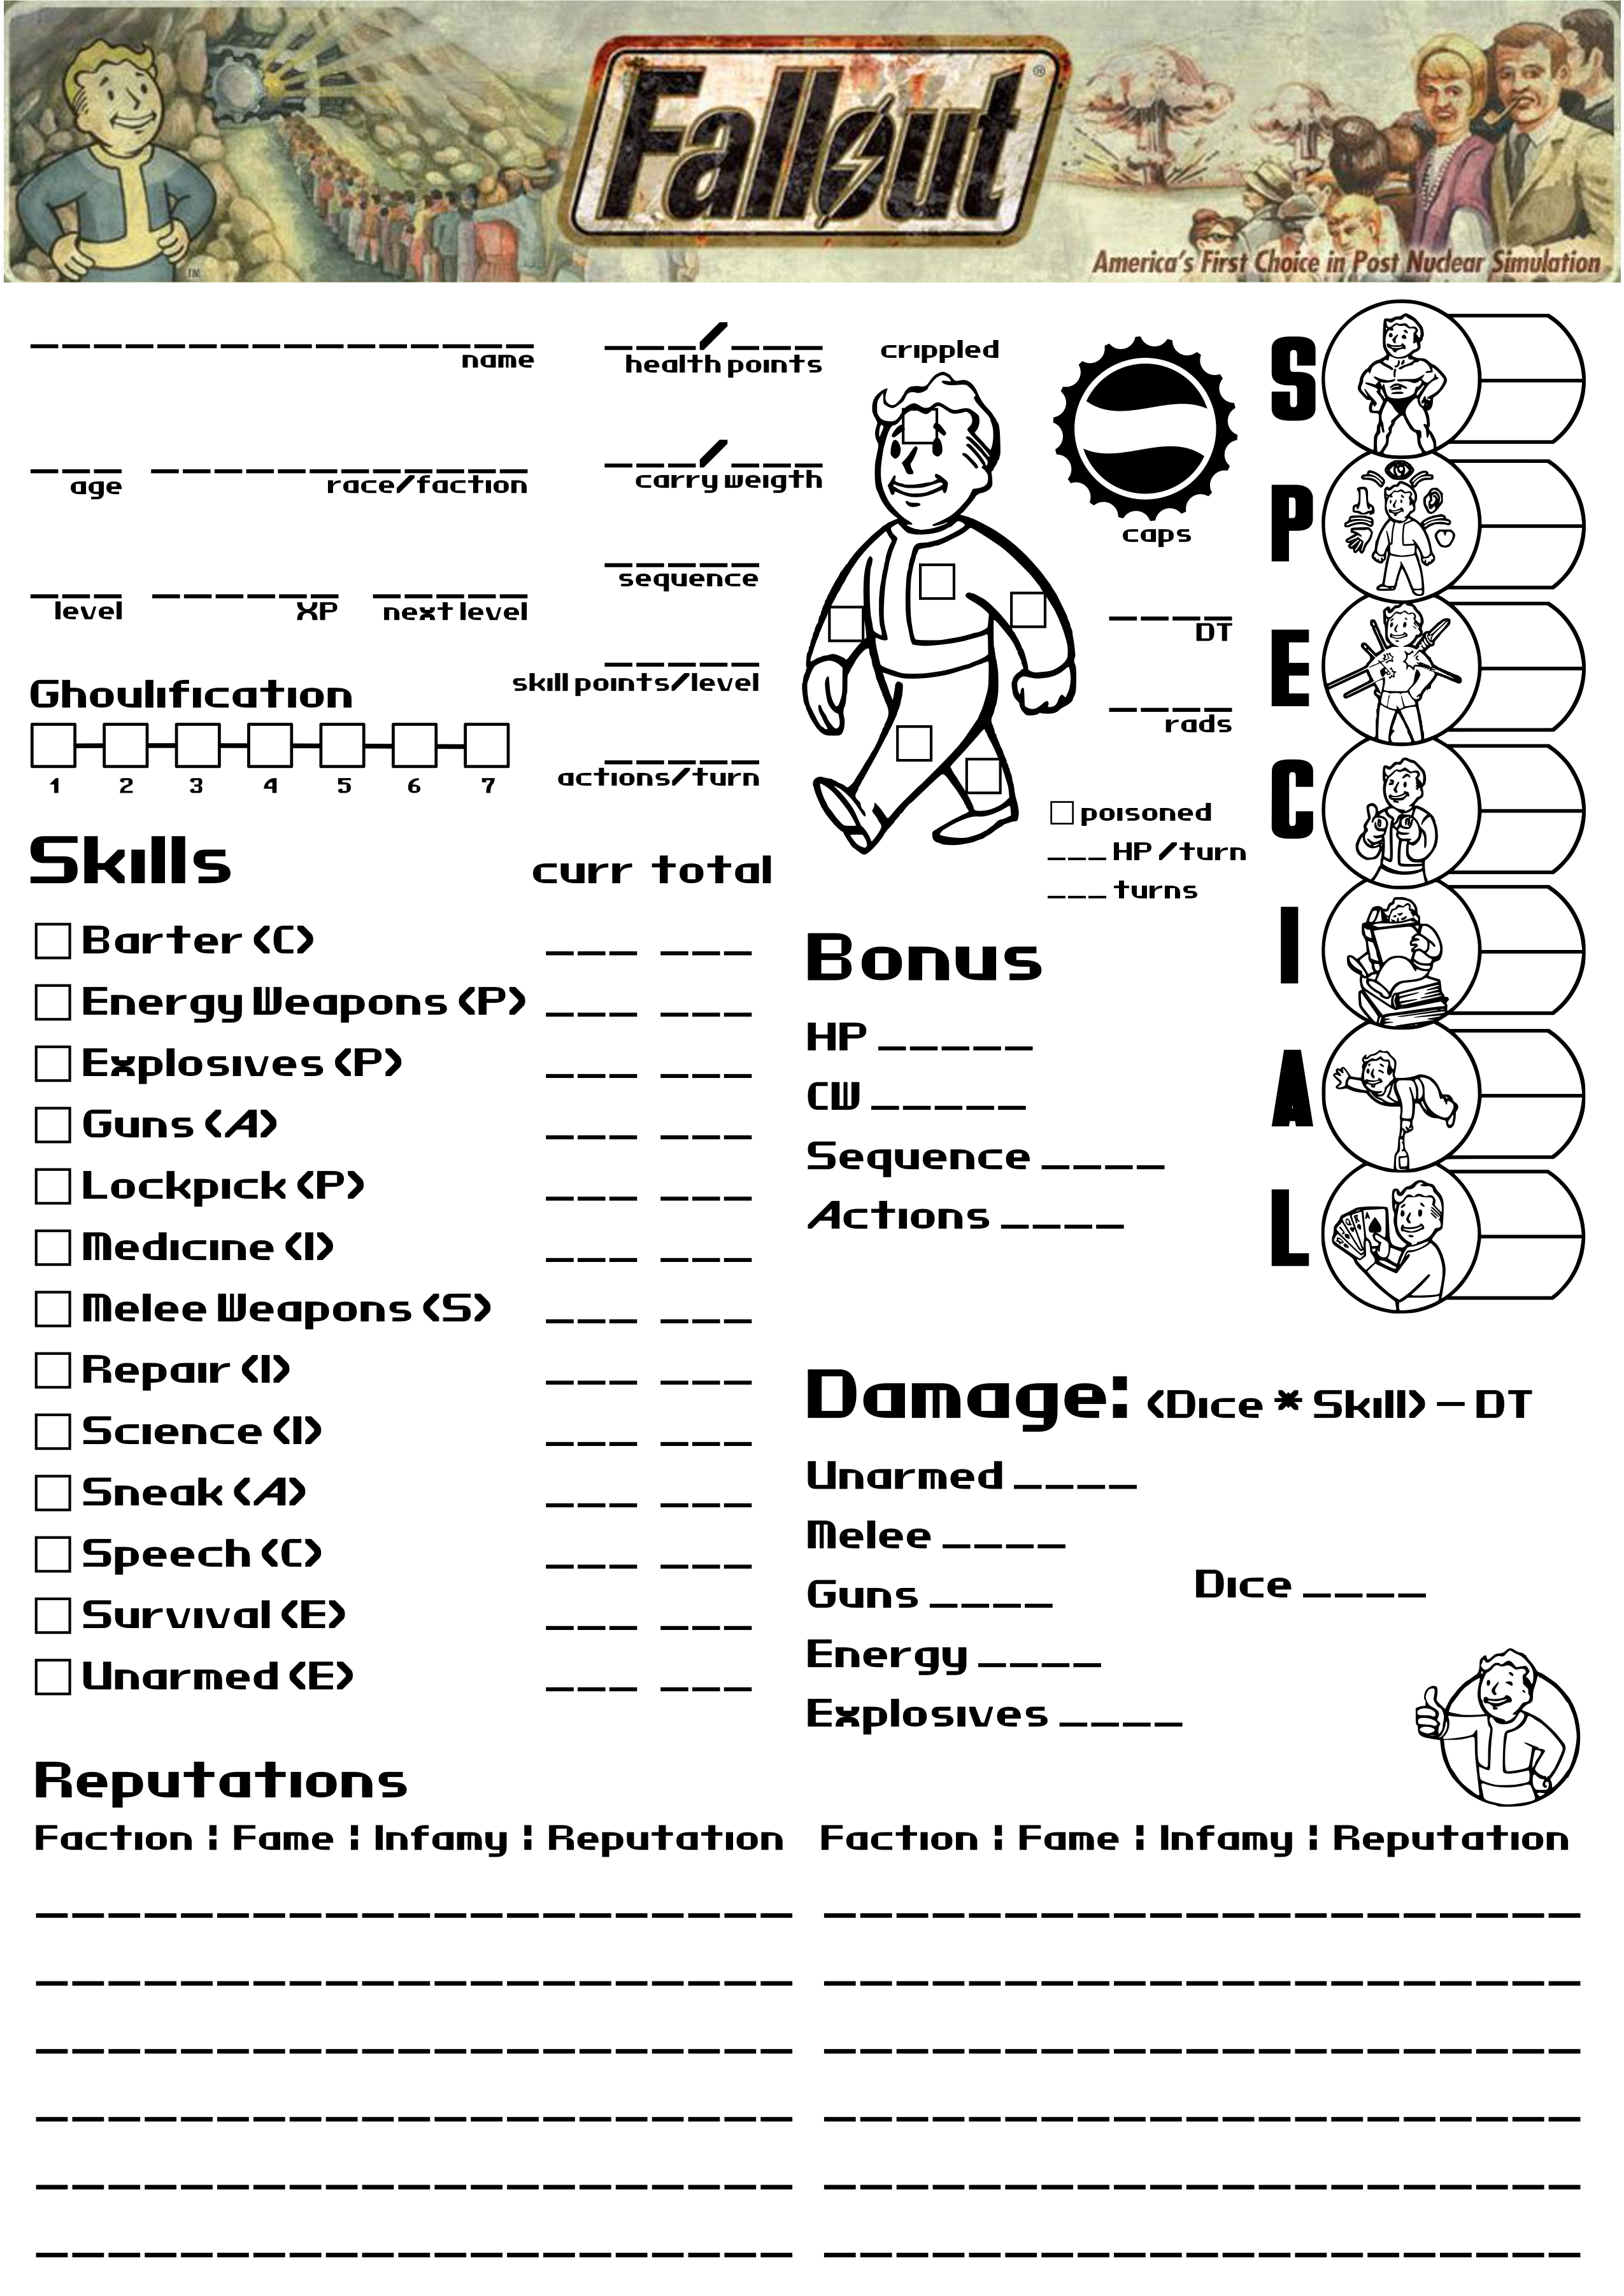
\includegraphics{char_sheet_p1_autofill}}}

\begin{Form}

%%%%%%%%%%%%%%%%%%%%%%
%%           S.P.E.C.I.A.L.
%%%%%%%%%%%%%%%%%%%%%%

\begin{textblock}{3}(14.55, 2)
\TextField[maxlen=2,align=2,height=15pt,width=23pt,name=Str,value=1]{}
\end{textblock}

\begin{textblock}{3}(14.55, 2.5)
\TextField[maxlen=2,align=2,height=15pt,width=23pt,name=BonusStr,value=0]{}
\end{textblock}

\begin{textblock}{3}(14.55, 3.05)
\TextField[maxlen=2,align=2,height=15pt,width=23pt,name=Per,value=1]{}
\end{textblock}

\begin{textblock}{3}(14.55, 3.5)
\TextField[maxlen=2,align=2,height=15pt,width=23pt,name=BonusPer,value=0]{}
\end{textblock}

\begin{textblock}{3}(14.55, 4.05)
\TextField[maxlen=2,align=2,height=15pt,width=23pt,name=End,value=1]{}
\end{textblock}

\begin{textblock}{3}(14.55, 4.5)
\TextField[maxlen=2,align=2,height=15pt,width=23pt,name=BonusEnd,value=0]{}
\end{textblock}

\begin{textblock}{3}(14.55, 5.05)
\TextField[maxlen=2,align=2,height=15pt,width=23pt,name=Cha,value=1]{}
\end{textblock}

\begin{textblock}{3}(14.55, 5.5)
\TextField[maxlen=2,align=2,height=15pt,width=23pt,name=BonusCha,value=0]{}
\end{textblock}

\begin{textblock}{3}(14.55, 6.05)
\TextField[maxlen=2,align=2,height=15pt,width=23pt,name=Int,value=1]{}
\end{textblock}

\begin{textblock}{3}(14.55, 6.5)
\TextField[maxlen=2,align=2,height=15pt,width=23pt,name=BonusInt,value=0]{}
\end{textblock}

\begin{textblock}{3}(14.55, 7.05)
\TextField[maxlen=2,align=2,height=15pt,width=23pt,name=Agi,value=1]{}
\end{textblock}

\begin{textblock}{3}(14.55, 7.5)
\TextField[maxlen=2,align=2,height=15pt,width=23pt,name=BonusAgi,value=0]{}
\end{textblock}

\begin{textblock}{3}(14.55, 8.05)
\TextField[maxlen=2,align=2,height=15pt,width=23pt,name=Luc,value=1]{}
\end{textblock}

\begin{textblock}{3}(14.55, 8.5)
\TextField[maxlen=2,align=2,height=15pt,width=23pt,name=BonusLuc,value=0]{}
\end{textblock}


%%%%%%%%%%%%%%%%%%%%%%
%%           BASIC DATA
%%%%%%%%%%%%%%%%%%%%%%

\begin{textblock}{3}(0.14, 1.85)
\TextField[maxlen=100,align=2,height=15pt,width=185pt,name=name]{}
\end{textblock}

\begin{textblock}{3}(0.14, 2.7)
\TextField[maxlen=4,align=2,height=15pt,width=35pt,name=age]{}
\end{textblock}

\begin{textblock}{3}(0.14, 3.6)
\TextField[maxlen=3,align=2,height=15pt,width=35pt,name=level,value=1]{}
\end{textblock}

\begin{textblock}{3}(1.3, 2.7)
\TextField[maxlen=100,align=2,height=15pt,width=140pt,name=racebg]{}
\end{textblock}

\begin{textblock}{3}(1.3, 3.6)
\TextField[maxlen=100,align=2,height=15pt,width=70pt,name=xp,value=0]{}
\end{textblock}

\begin{textblock}{3}(3.45, 3.6)
\TextField[calculate={%
    var f_level= this.getField("level");
    event.value = 25 * ((3 * f_level.value + 3) + 2) * (f_level.value);
  },maxlen=4,align=2,height=15pt,width=60pt,name=nextLevel,value=200]{}
\end{textblock}

\begin{textblock}{3}(5.75, 1.85)
\TextField[maxlen=4,align=2,height=15pt,width=35pt,name=hpcurr,value=0]{}
\end{textblock}
\begin{textblock}{3}(7.1, 1.85)
\TextField[calculate={%
    var f_End = this.getField("End");
    var f_BonusEnd = this.getField("BonusEnd");
    var f_Level = this.getField("level");
    var f_bonushp = this.getField("bonushp");
    event.value = 100 + ((f_End.value + f_BonusEnd.value) * 20) + f_bonushp.value + ((f_Level.value - 1) * 5);
  },maxlen=4,align=2,height=15pt,width=35pt,name=hpmax]{}
\end{textblock}

\begin{textblock}{3}(5.75, 2.68)
\TextField[maxlen=3,align=2,height=15pt,width=35pt,name=cwcurr,value=0]{}
\end{textblock}
\begin{textblock}{3}(7.1, 2.68)
\TextField[calculate={%
    var f_Str = this.getField("Str");
    var f_BonusStr = this.getField("BonusStr");
    var f_bonuscw = this.getField("bonuscw");
    event.value = 150 + ((f_Str.value + f_BonusStr.value) * 10) + f_bonuscw.value;
  },maxlen=3,align=2,height=15pt,width=35pt,name=cwmax]{}
\end{textblock}

\begin{textblock}{3}(5.75, 3.37)
\TextField[maxlen=3,align=2,height=15pt,width=60pt,name=sequence,value=0]{}
\end{textblock}

\begin{textblock}{3}(5.75, 4.08)
\TextField[calculate={%
    var f_Int = this.getField("Int");
    var f_BonusInt = this.getField("BonusInt");
    event.value = 10 + Math.ceil((f_Int.value + f_BonusInt.value) / 2);
  },maxlen=3,align=2,height=15pt,width=60pt,name=skillpointsperlevel,readonly=true]{}
\end{textblock}

\begin{textblock}{3}(5.75, 4.76)
\TextField[calculate={%
    var f_Agi = this.getField("Agi");
    var f_BonusAgi = this.getField("BonusAgi");
    var f_bonusact = this.getField("bonusact");
    event.value = Math.ceil((f_Agi.value + f_BonusAgi.value) / 2) + f_bonusact.value;
  },maxlen=3,align=2,height=15pt,width=60pt,name=actionsperturn,readonly=true]{}
\end{textblock}

\begin{textblock}{3}(10.7, 2.6)
\TextField[maxlen=100,align=2,height=15pt,width=35pt,name=caps,value=0]{}
\end{textblock}

\begin{textblock}{3}(10.8, 3.75)
\TextField[maxlen=100,align=2,height=15pt,width=45pt,name=dt,value=0]{}
\end{textblock}

\begin{textblock}{3}(10.8, 4.4)
\TextField[maxlen=100,align=2,height=15pt,width=45pt,name=rads,value=0]{}
\end{textblock}

%%%%%%%%%%%%%%%%%%%%%%
%%           GHOULIFICATION
%%%%%%%%%%%%%%%%%%%%%%

\begin{textblock}{1}(0.14, 4.83)
\CheckBox[width=1.4em,name=ghoulification1]{}
\end{textblock}

\begin{textblock}{1}(0.86, 4.83)
\CheckBox[width=1.4em,name=ghoulification2]{}
\end{textblock}

\begin{textblock}{1}(1.58, 4.83)
\CheckBox[width=1.4em,name=ghoulification3]{}
\end{textblock}

\begin{textblock}{1}(2.30, 4.83)
\CheckBox[width=1.4em,name=ghoulification4]{}
\end{textblock}

\begin{textblock}{1}(3.02, 4.83)
\CheckBox[width=1.4em,name=ghoulification5]{}
\end{textblock}

\begin{textblock}{1}(3.74, 4.83)
\CheckBox[width=1.4em,name=ghoulification6]{}
\end{textblock}

\begin{textblock}{1}(4.46, 4.83)
\CheckBox[width=1.4em,name=ghoulification7]{}
\end{textblock}

%%%%%%%%%%%%%%%%%%%%%%
%%           CRIPPLED
%%%%%%%%%%%%%%%%%%%%%%

\begin{textblock}{1}(8.8, 2.6)
\CheckBox[width=0.9em,height=0.9em,name=crippledHead]{}
\end{textblock}

\begin{textblock}{1}(8.05, 4)
\CheckBox[width=0.9em,height=0.9em,name=crippledLArm]{}
\end{textblock}

\begin{textblock}{1}(8.97, 3.68)
\CheckBox[width=0.9em,height=0.9em,name=crippledTorso]{}
\end{textblock}

\begin{textblock}{1}(9.87, 3.87)
\CheckBox[width=0.9em,height=0.9em,name=crippledRArm]{}
\end{textblock}

\begin{textblock}{1}(9.4, 5.05)
\CheckBox[width=0.9em,height=0.9em,name=crippledLLeg]{}
\end{textblock}

\begin{textblock}{1}(8.75, 4.83)
\CheckBox[width=0.9em,height=0.9em,name=crippledRLeg]{}
\end{textblock}

%%%%%%%%%%%%%%%%%%%%%%
%%           POISON
%%%%%%%%%%%%%%%%%%%%%%

\begin{textblock}{1}(10.15, 5.28)
\CheckBox[width=0.9em,height=0.9em,name=poison]{}
\end{textblock}

\begin{textblock}{3}(10.15, 5.54)
\TextField[maxlen=3,align=2,height=10pt,width=25pt,name=hpperturn]{}
\end{textblock}

\begin{textblock}{3}(10.15, 5.81)
\TextField[maxlen=3,align=2,height=10pt,width=25pt,name=turns]{}
\end{textblock}

%%%%%%%%%%%%%%%%%%%%%%
%%           BONUS
%%%%%%%%%%%%%%%%%%%%%%

\begin{textblock}{3}(8.55,6.76)
\TextField[maxlen=3,align=2,height=15pt,width=55pt,name=bonushp,value=0]{}
\end{textblock}

\begin{textblock}{3}(8.49,7.17)
\TextField[maxlen=3,align=2,height=15pt,width=55pt,name=bonuscw,value=0]{}
\end{textblock}

\begin{textblock}{3}(10.17,7.59)
\TextField[maxlen=3,align=2,height=15pt,width=45pt,name=bonusseq,value=0]{}
\end{textblock}

\begin{textblock}{3}(9.76,8.01)
\TextField[maxlen=3,align=2,height=15pt,width=45pt,name=bonusact,value=0]{}
\end{textblock}

%%%%%%%%%%%%%%%%%%%%%%
%%           DAMAGE CALCULATION
%%%%%%%%%%%%%%%%%%%%%%

\begin{textblock}{3}(12.72,10.58)
\TextField[maxlen=3,align=2,height=15pt,width=45pt,name=dicedamage,value=0]{}
\end{textblock}

\begin{textblock}{3}(9.87,9.84)
\TextField[
  maxlen=40,
  calculate={%
    var f_Str = this.getField("Str");
    var f_BonusStr = this.getField("BonusStr");
    var f_skillUnarmed = this.getField("skillUnarmed");
    event.value = Math.ceil(((f_skillUnarmed.value + 50) / 100) * (f_Str.value + f_BonusStr.value));
  },
   align=2,height=15pt,width=45pt,name=dmgUnarmed,readonly=true]{}
\end{textblock}

\begin{textblock}{3}(9.2,10.27)
\TextField[
  maxlen=40,
  calculate={%
    var f_Str = this.getField("Str");
    var f_BonusStr = this.getField("BonusStr");
    var f_dice = this.getField("dicedamage");
    event.value = f_dice.value + Math.ceil((f_Str.value + f_BonusStr.value) / 2);
  },
   align=2,height=15pt,width=45pt,name=dmgMelee,readonly=true]{}
\end{textblock}

\begin{textblock}{3}(9.08,10.68)
\TextField[
  maxlen=40,
  calculate={%
    var f_skillGuns = this.getField("skillGuns");
    var f_dice = this.getField("dicedamage");
    event.value = Math.ceil(f_dice.value * ((f_skillGuns.value + 50) / 100));
  },
   align=2,height=15pt,width=45pt,name=dmgGuns,readonly=true]{}
\end{textblock}

\begin{textblock}{3}(9.5,11.1)
\TextField[
  maxlen=40,
  calculate={%
    var f_skillEnergy = this.getField("skillEnergy");
    var f_dice = this.getField("dicedamage");
    event.value = Math.ceil(f_dice.value * ((f_skillEnergy.value + 50) / 100));
  },
   align=2,height=15pt,width=45pt,name=dmgEnergy,readonly=true]{}
\end{textblock}

\begin{textblock}{3}(10.3,11.51)
\TextField[
  maxlen=40,
  calculate={%
    var f_skillExplosives = this.getField("skillExplosives");
    var f_dice = this.getField("dicedamage");
    event.value = Math.ceil(f_dice.value * ((f_skillExplosives.value + 50) / 100));
  },
   align=2,height=15pt,width=45pt,name=dmgExplosives,readonly=true]{}
\end{textblock}

%%%%%%%%%%%%%%%%%%%%%%
%%           SKILLS AND BONUS
%%%%%%%%%%%%%%%%%%%%%%
\begin{textblock}{1}(0.14,6.23)
\CheckBox[width=1em,height=1em,name=tagBarter]{}
\end{textblock}
\begin{textblock}{3}(5.16,6.19)
\TextField[maxlen=3,align=2,height=15pt,width=35pt,name=skillBarter,value=0]{}
\end{textblock}
\begin{textblock}{3}(6.35,6.19)
\TextField[calculate={%
    var f_base = this.getField("skillBarter");
    var f_Skill = this.getField("Cha");
    var f_bSkill = this.getField("BonusCha");
    var f_Luck = this.getField("Luc");
    var f_bLuck = this.getField("BonusLuc");
    event.value = f_base.value + 2 + (2 * (f_Skill.value + f_bSkill.value)) + Math.ceil((f_Luck.value + f_bLuck.value) / 2);
  },maxlen=3,align=2,height=15pt,width=35pt,name=finalBarter,readonly=true]{}
\end{textblock}

\begin{textblock}{1}(0.14,6.65)
\CheckBox[width=1em,height=1em,name=tagEnergy]{}
\end{textblock}
\begin{textblock}{3}(5.16,6.60)
\TextField[maxlen=3,align=2,height=15pt,width=35pt,name=skillEnergy,value=0]{}
\end{textblock}
\begin{textblock}{3}(6.35,6.60)
\TextField[calculate={%
    var f_base = this.getField("skillEnergy");
    var f_Skill = this.getField("Per");
    var f_bSkill = this.getField("BonusPer");
    var f_Luck = this.getField("Luc");
    var f_bLuck = this.getField("BonusLuc");
    event.value = f_base.value + 2 + (2 * (f_Skill.value + f_bSkill.value)) + Math.ceil((f_Luck.value + f_bLuck.value) / 2);
  },maxlen=3,align=2,height=15pt,width=35pt,name=finalEnergy,readonly=true]{}
\end{textblock}

\begin{textblock}{1}(0.14,7.08)
\CheckBox[width=1em,height=1em,name=tagExplosives]{}
\end{textblock}
\begin{textblock}{3}(5.16,7.03)
\TextField[maxlen=3,align=2,height=15pt,width=35pt,name=skillExplosives,value=0]{}
\end{textblock}
\begin{textblock}{3}(6.35,7.03)
\TextField[calculate={%
    var f_base = this.getField("skillExplosives");
    var f_Skill = this.getField("Per");
    var f_bSkill = this.getField("BonusPer");
    var f_Luck = this.getField("Luc");
    var f_bLuck = this.getField("BonusLuc");
    event.value = f_base.value + 2 + (2 * (f_Skill.value + f_bSkill.value)) + Math.ceil((f_Luck.value + f_bLuck.value) / 2);
  },maxlen=3,align=2,height=15pt,width=35pt,name=finalExplosives,readonly=true]{}
\end{textblock}

\begin{textblock}{1}(0.14,7.52)
\CheckBox[width=1em,height=1em,name=tagGuns]{}
\end{textblock}
\begin{textblock}{3}(5.16,7.46)
\TextField[maxlen=3,align=2,height=15pt,width=35pt,name=skillGuns,value=0]{}
\end{textblock}
\begin{textblock}{3}(6.35,7.46)
\TextField[calculate={%
    var f_base = this.getField("skillGuns");
    var f_Skill = this.getField("Agi");
    var f_bSkill = this.getField("BonusAgi");
    var f_Luck = this.getField("Luc");
    var f_bLuck = this.getField("BonusLuc");
    event.value = f_base.value + 2 + (2 * (f_Skill.value + f_bSkill.value)) + Math.ceil((f_Luck.value + f_bLuck.value) / 2);
  },maxlen=3,align=2,height=15pt,width=35pt,name=finalGuns,readonly=true]{}
\end{textblock}

\begin{textblock}{1}(0.14,7.96)
\CheckBox[width=1em,height=1em,name=tagLockpick]{}
\end{textblock}
\begin{textblock}{3}(5.16,7.89)
\TextField[maxlen=3,align=2,height=15pt,width=35pt,name=skillLockpick,value=0]{}
\end{textblock}
\begin{textblock}{3}(6.35,7.89)
\TextField[calculate={%
    var f_base = this.getField("skillLockpick");
    var f_Skill = this.getField("Per");
    var f_bSkill = this.getField("BonusPer");
    var f_Luck = this.getField("Luc");
    var f_bLuck = this.getField("BonusLuc");
    event.value = f_base.value + 2 + (2 * (f_Skill.value + f_bSkill.value)) + Math.ceil((f_Luck.value + f_bLuck.value) / 2);
  },maxlen=3,align=2,height=15pt,width=35pt,name=finalLockpick,readonly=true]{}
\end{textblock}

\begin{textblock}{1}(0.14,8.41)
\CheckBox[width=1em,height=1em,name=tagMedicine]{}
\end{textblock}
\begin{textblock}{3}(5.16,8.33)
\TextField[maxlen=3,align=2,height=15pt,width=35pt,name=skillMedicine,value=0]{}
\end{textblock}
\begin{textblock}{3}(6.35,8.33)
\TextField[calculate={%
    var f_base = this.getField("skillMedicine");
    var f_Skill = this.getField("Int");
    var f_bSkill = this.getField("BonusInt");
    var f_Luck = this.getField("Luc");
    var f_bLuck = this.getField("BonusLuc");
    event.value = f_base.value + 2 + (2 * (f_Skill.value + f_bSkill.value)) + Math.ceil((f_Luck.value + f_bLuck.value) / 2);
  },maxlen=3,align=2,height=15pt,width=35pt,name=finalMedicine,readonly=true]{}
\end{textblock}

\begin{textblock}{1}(0.14,8.85)
\CheckBox[width=1em,height=1em,name=tagMelee]{}
\end{textblock}
\begin{textblock}{3}(5.16,8.75)
\TextField[maxlen=3,align=2,height=15pt,width=35pt,name=skillMelee,value=0]{}
\end{textblock}
\begin{textblock}{3}(6.35,8.75)
\TextField[calculate={%
    var f_base = this.getField("skillMelee");
    var f_Skill = this.getField("Cha");
    var f_bSkill = this.getField("BonusCha");
    var f_Luck = this.getField("Luc");
    var f_bLuck = this.getField("BonusLuc");
    event.value = f_base.value + 2 + (2 * (f_Skill.value + f_bSkill.value)) + Math.ceil((f_Luck.value + f_bLuck.value) / 2);
  },maxlen=3,align=2,height=15pt,width=35pt,name=finalMelee,readonly=true]{}
\end{textblock}

\begin{textblock}{1}(0.14,9.29)
\CheckBox[width=1em,height=1em,name=tagRepair]{}
\end{textblock}
\begin{textblock}{3}(5.16,9.19)
\TextField[maxlen=3,align=2,height=15pt,width=35pt,name=skillRepair,value=0]{}
\end{textblock}
\begin{textblock}{3}(6.35,9.19)
\TextField[calculate={%
    var f_base = this.getField("skillRepair");
    var f_Skill = this.getField("Cha");
    var f_bSkill = this.getField("BonusCha");
    var f_Luck = this.getField("Luc");
    var f_bLuck = this.getField("BonusLuc");
    event.value = f_base.value + 2 + (2 * (f_Skill.value + f_bSkill.value)) + Math.ceil((f_Luck.value + f_bLuck.value) / 2);
  },maxlen=3,align=2,height=15pt,width=35pt,name=finalRepair,readonly=true]{}
\end{textblock}

\begin{textblock}{1}(0.14,9.72)
\CheckBox[width=1em,height=1em,name=tagScience]{}
\end{textblock}
\begin{textblock}{3}(5.16,9.62)
\TextField[maxlen=3,align=2,height=15pt,width=35pt,name=skillScience,value=0]{}
\end{textblock}
\begin{textblock}{3}(6.35,9.62)
\TextField[calculate={%
    var f_base = this.getField("skillScience");
    var f_Skill = this.getField("Cha");
    var f_bSkill = this.getField("BonusCha");
    var f_Luck = this.getField("Luc");
    var f_bLuck = this.getField("BonusLuc");
    event.value = f_base.value + 2 + (2 * (f_Skill.value + f_bSkill.value)) + Math.ceil((f_Luck.value + f_bLuck.value) / 2);
  },maxlen=3,align=2,height=15pt,width=35pt,name=finalScience,readonly=true]{}
\end{textblock}

\begin{textblock}{1}(0.14,10.15)
\CheckBox[width=1em,height=1em,name=tagSneak]{}
\end{textblock}
\begin{textblock}{3}(5.16,10.06)
\TextField[maxlen=3,align=2,height=15pt,width=35pt,name=skillSneak,value=0]{}
\end{textblock}
\begin{textblock}{3}(6.35,10.06)
\TextField[calculate={%
    var f_base = this.getField("skillSneak");
    var f_Skill = this.getField("Agi");
    var f_bSkill = this.getField("BonusAgi");
    var f_Luck = this.getField("Luc");
    var f_bLuck = this.getField("BonusLuc");
    event.value = f_base.value + 2 + (2 * (f_Skill.value + f_bSkill.value)) + Math.ceil((f_Luck.value + f_bLuck.value) / 2);
  },maxlen=3,align=2,height=15pt,width=35pt,name=finalSneak,readonly=true]{}
\end{textblock}

\begin{textblock}{1}(0.14,10.57)
\CheckBox[width=1em,height=1em,name=tagSpeech]{}
\end{textblock}
\begin{textblock}{3}(5.16,10.47)
\TextField[maxlen=3,align=2,height=15pt,width=35pt,name=skillSpeech,value=0]{}
\end{textblock}
\begin{textblock}{3}(6.35,10.47)
\TextField[calculate={%
    var f_base = this.getField("skillSpeech");
    var f_Skill = this.getField("Cha");
    var f_bSkill = this.getField("BonusCha");
    var f_Luck = this.getField("Luc");
    var f_bLuck = this.getField("BonusLuc");
    event.value = f_base.value + 2 + (2 * (f_Skill.value + f_bSkill.value)) + Math.ceil((f_Luck.value + f_bLuck.value) / 2);
  },maxlen=3,align=2,height=15pt,width=35pt,name=finalSpeech,readonly=true]{}
\end{textblock}

\begin{textblock}{1}(0.14,11.01)
\CheckBox[width=1em,height=1em,name=tagSurvival]{}
\end{textblock}
\begin{textblock}{3}(5.16,10.91)
\TextField[maxlen=3,align=2,height=15pt,width=35pt,name=skillSurvival,value=0]{}
\end{textblock}
\begin{textblock}{3}(6.35,10.91)
\TextField[calculate={%
    var f_base = this.getField("skillSurvival");
    var f_Skill = this.getField("Cha");
    var f_bSkill = this.getField("BonusCha");
    var f_Luck = this.getField("Luc");
    var f_bLuck = this.getField("BonusLuc");
    event.value = f_base.value + 2 + (2 * (f_Skill.value + f_bSkill.value)) + Math.ceil((f_Luck.value + f_bLuck.value) / 2);
  },maxlen=3,align=2,height=15pt,width=35pt,name=finalSurvival,readonly=true]{}
\end{textblock}

\begin{textblock}{1}(0.14,11.42)
\CheckBox[width=1em,height=1em,name=tagUnarmed]{}
\end{textblock}
\begin{textblock}{3}(5.16,11.35)
\TextField[maxlen=3,align=2,height=15pt,width=35pt,name=skillUnarmed,value=0]{}
\end{textblock}
\begin{textblock}{3}(6.35,11.35)
\TextField[calculate={%
    var f_base = this.getField("skillUnarmed");
    var f_Skill = this.getField("Cha");
    var f_bSkill = this.getField("BonusCha");
    var f_Luck = this.getField("Luc");
    var f_bLuck = this.getField("BonusLuc");
    event.value = f_base.value + 2 + (2 * (f_Skill.value + f_bSkill.value)) + Math.ceil((f_Luck.value + f_bLuck.value) / 2);
  },maxlen=3,align=2,height=15pt,width=35pt,name=finalUnarmed,readonly=true]{}
\end{textblock}

%%%%%%%%%%%%%%%%%%%%%%
%%           REPUTATIONS
%%%%%%%%%%%%%%%%%%%%%%

\begin{textblock}{3}(0.14, 12.87)
\TextField[maxlen=100,align=2,height=15pt,width=60pt,name=reputationFaction1]{}
\end{textblock}
\begin{textblock}{3}(2.05, 12.87)
\TextField[maxlen=100,align=2,height=15pt,width=30pt,name=reputationFame1]{}
\end{textblock}
\begin{textblock}{3}(3.14, 12.87)
\TextField[maxlen=100,align=2,height=15pt,width=30pt,name=reputationInfamy1]{}
\end{textblock}
\begin{textblock}{3}(4.29, 12.87)
\TextField[calculate={%
var f_fame = this.getField("reputationFame1");
var f_infamy = this.getField("reputationInfamy1");
if (f_fame.value == 1 && f_infamy.value == 1)
	event.value = "Neutral";
else if (f_fame.value == 2 && f_infamy.value == 1)
	event.value = "Accepted";
else if (f_fame.value == 3 && f_infamy.value == 1)
	event.value = "Liked";
else if (f_fame.value == 4 && f_infamy.value == 1)
	event.value = "Idolized";
else if (f_fame.value == 1 && f_infamy.value == 2)
	event.value = "Shunned";
else if (f_fame.value == 2 && f_infamy.value == 2)
	event.value = "Mixed";
else if (f_fame.value == 3 && f_infamy.value == 2)
	event.value = "Smiling Troublemaker";
else if (f_fame.value == 4 && f_infamy.value == 2)
	event.value = "Good-Natured Rascal";
else if (f_fame.value == 1 && f_infamy.value == 3)
	event.value = "Hated";
else if (f_fame.value == 2 && f_infamy.value == 3)
	event.value = "Sneering Punk";
else if (f_fame.value == 3 && f_infamy.value == 3)
	event.value = "Unpredictable";
else if (f_fame.value == 4 && f_infamy.value == 3)
	event.value = "Dark Hero";
else if (f_fame.value == 1 && f_infamy.value == 4)
	event.value = "Vilified";
else if (f_fame.value == 2 && f_infamy.value == 4)
	event.value = "Merciful Thug";
else if (f_fame.value == 3 && f_infamy.value == 4)
	event.value = "Soft-Hearted Devil";
else if (f_fame.value == 4 && f_infamy.value == 4)
	event.value = "Wild Child";
else
	event.value = "";
},maxlen=100,align=2,height=15pt,width=125pt,name=reputation1]{}
\end{textblock}

\begin{textblock}{3}(0.14, 13.33)
\TextField[maxlen=100,align=2,height=15pt,width=62pt,name=reputationFaction2]{}
\end{textblock}
\begin{textblock}{3}(2.05, 13.33)
\TextField[maxlen=100,align=2,height=15pt,width=30pt,name=reputationFame2]{}
\end{textblock}
\begin{textblock}{3}(3.14, 13.33)
\TextField[maxlen=100,align=2,height=15pt,width=30pt,name=reputationInfamy2]{}
\end{textblock}
\begin{textblock}{3}(4.29, 13.33)
\TextField[calculate={%
var f_fame = this.getField("reputationFame2");
var f_infamy = this.getField("reputationInfamy2");
if (f_fame.value == 1 && f_infamy.value == 1)
	event.value = "Neutral";
else if (f_fame.value == 2 && f_infamy.value == 1)
	event.value = "Accepted";
else if (f_fame.value == 3 && f_infamy.value == 1)
	event.value = "Liked";
else if (f_fame.value == 4 && f_infamy.value == 1)
	event.value = "Idolized";
else if (f_fame.value == 1 && f_infamy.value == 2)
	event.value = "Shunned";
else if (f_fame.value == 2 && f_infamy.value == 2)
	event.value = "Mixed";
else if (f_fame.value == 3 && f_infamy.value == 2)
	event.value = "Smiling Troublemaker";
else if (f_fame.value == 4 && f_infamy.value == 2)
	event.value = "Good-Natured Rascal";
else if (f_fame.value == 1 && f_infamy.value == 3)
	event.value = "Hated";
else if (f_fame.value == 2 && f_infamy.value == 3)
	event.value = "Sneering Punk";
else if (f_fame.value == 3 && f_infamy.value == 3)
	event.value = "Unpredictable";
else if (f_fame.value == 4 && f_infamy.value == 3)
	event.value = "Dark Hero";
else if (f_fame.value == 1 && f_infamy.value == 4)
	event.value = "Vilified";
else if (f_fame.value == 2 && f_infamy.value == 4)
	event.value = "Merciful Thug";
else if (f_fame.value == 3 && f_infamy.value == 4)
	event.value = "Soft-Hearted Devil";
else if (f_fame.value == 4 && f_infamy.value == 4)
	event.value = "Wild Child";
else
	event.value = "";
},maxlen=100,align=2,height=15pt,width=125pt,name=reputation2]{}
\end{textblock}

\begin{textblock}{3}(0.14, 13.8)
\TextField[maxlen=100,align=2,height=15pt,width=62pt,name=reputationFaction3]{}
\end{textblock}
\begin{textblock}{3}(2.05, 13.8)
\TextField[maxlen=100,align=2,height=15pt,width=30pt,name=reputationFame3]{}
\end{textblock}
\begin{textblock}{3}(3.14, 13.8)
\TextField[maxlen=100,align=2,height=15pt,width=30pt,name=reputationInfamy3]{}
\end{textblock}
\begin{textblock}{3}(4.29, 13.8)
\TextField[calculate={%
var f_fame = this.getField("reputationFame3");
var f_infamy = this.getField("reputationInfamy3");
if (f_fame.value == 1 && f_infamy.value == 1)
	event.value = "Neutral";
else if (f_fame.value == 2 && f_infamy.value == 1)
	event.value = "Accepted";
else if (f_fame.value == 3 && f_infamy.value == 1)
	event.value = "Liked";
else if (f_fame.value == 4 && f_infamy.value == 1)
	event.value = "Idolized";
else if (f_fame.value == 1 && f_infamy.value == 2)
	event.value = "Shunned";
else if (f_fame.value == 2 && f_infamy.value == 2)
	event.value = "Mixed";
else if (f_fame.value == 3 && f_infamy.value == 2)
	event.value = "Smiling Troublemaker";
else if (f_fame.value == 4 && f_infamy.value == 2)
	event.value = "Good-Natured Rascal";
else if (f_fame.value == 1 && f_infamy.value == 3)
	event.value = "Hated";
else if (f_fame.value == 2 && f_infamy.value == 3)
	event.value = "Sneering Punk";
else if (f_fame.value == 3 && f_infamy.value == 3)
	event.value = "Unpredictable";
else if (f_fame.value == 4 && f_infamy.value == 3)
	event.value = "Dark Hero";
else if (f_fame.value == 1 && f_infamy.value == 4)
	event.value = "Vilified";
else if (f_fame.value == 2 && f_infamy.value == 4)
	event.value = "Merciful Thug";
else if (f_fame.value == 3 && f_infamy.value == 4)
	event.value = "Soft-Hearted Devil";
else if (f_fame.value == 4 && f_infamy.value == 4)
	event.value = "Wild Child";
else
	event.value = "";
},maxlen=100,align=2,height=15pt,width=125pt,name=reputation3]{}
\end{textblock}

\begin{textblock}{3}(0.14, 14.28)
\TextField[maxlen=100,align=2,height=15pt,width=62pt,name=reputationFaction4]{}
\end{textblock}
\begin{textblock}{3}(2.05, 14.28)
\TextField[maxlen=100,align=2,height=15pt,width=30pt,name=reputationFame4]{}
\end{textblock}
\begin{textblock}{3}(3.14, 14.28)
\TextField[maxlen=100,align=2,height=15pt,width=30pt,name=reputationInfamy4]{}
\end{textblock}
\begin{textblock}{3}(4.29, 14.28)
\TextField[calculate={%
var f_fame = this.getField("reputationFame4");
var f_infamy = this.getField("reputationInfamy4");
if (f_fame.value == 1 && f_infamy.value == 1)
	event.value = "Neutral";
else if (f_fame.value == 2 && f_infamy.value == 1)
	event.value = "Accepted";
else if (f_fame.value == 3 && f_infamy.value == 1)
	event.value = "Liked";
else if (f_fame.value == 4 && f_infamy.value == 1)
	event.value = "Idolized";
else if (f_fame.value == 1 && f_infamy.value == 2)
	event.value = "Shunned";
else if (f_fame.value == 2 && f_infamy.value == 2)
	event.value = "Mixed";
else if (f_fame.value == 3 && f_infamy.value == 2)
	event.value = "Smiling Troublemaker";
else if (f_fame.value == 4 && f_infamy.value == 2)
	event.value = "Good-Natured Rascal";
else if (f_fame.value == 1 && f_infamy.value == 3)
	event.value = "Hated";
else if (f_fame.value == 2 && f_infamy.value == 3)
	event.value = "Sneering Punk";
else if (f_fame.value == 3 && f_infamy.value == 3)
	event.value = "Unpredictable";
else if (f_fame.value == 4 && f_infamy.value == 3)
	event.value = "Dark Hero";
else if (f_fame.value == 1 && f_infamy.value == 4)
	event.value = "Vilified";
else if (f_fame.value == 2 && f_infamy.value == 4)
	event.value = "Merciful Thug";
else if (f_fame.value == 3 && f_infamy.value == 4)
	event.value = "Soft-Hearted Devil";
else if (f_fame.value == 4 && f_infamy.value == 4)
	event.value = "Wild Child";
else
	event.value = "";
},maxlen=100,align=2,height=15pt,width=125pt,name=reputation4]{}
\end{textblock}

\begin{textblock}{3}(0.14, 14.74)
\TextField[maxlen=100,align=2,height=15pt,width=62pt,name=reputationFaction5]{}
\end{textblock}
\begin{textblock}{3}(2.05, 14.74)
\TextField[maxlen=100,align=2,height=15pt,width=30pt,name=reputationFame5]{}
\end{textblock}
\begin{textblock}{3}(3.14, 14.74)
\TextField[maxlen=100,align=2,height=15pt,width=30pt,name=reputationInfamy5]{}
\end{textblock}
\begin{textblock}{3}(4.29, 14.74)
\TextField[calculate={%
var f_fame = this.getField("reputationFame5");
var f_infamy = this.getField("reputationInfamy5");
if (f_fame.value == 1 && f_infamy.value == 1)
	event.value = "Neutral";
else if (f_fame.value == 2 && f_infamy.value == 1)
	event.value = "Accepted";
else if (f_fame.value == 3 && f_infamy.value == 1)
	event.value = "Liked";
else if (f_fame.value == 4 && f_infamy.value == 1)
	event.value = "Idolized";
else if (f_fame.value == 1 && f_infamy.value == 2)
	event.value = "Shunned";
else if (f_fame.value == 2 && f_infamy.value == 2)
	event.value = "Mixed";
else if (f_fame.value == 3 && f_infamy.value == 2)
	event.value = "Smiling Troublemaker";
else if (f_fame.value == 4 && f_infamy.value == 2)
	event.value = "Good-Natured Rascal";
else if (f_fame.value == 1 && f_infamy.value == 3)
	event.value = "Hated";
else if (f_fame.value == 2 && f_infamy.value == 3)
	event.value = "Sneering Punk";
else if (f_fame.value == 3 && f_infamy.value == 3)
	event.value = "Unpredictable";
else if (f_fame.value == 4 && f_infamy.value == 3)
	event.value = "Dark Hero";
else if (f_fame.value == 1 && f_infamy.value == 4)
	event.value = "Vilified";
else if (f_fame.value == 2 && f_infamy.value == 4)
	event.value = "Merciful Thug";
else if (f_fame.value == 3 && f_infamy.value == 4)
	event.value = "Soft-Hearted Devil";
else if (f_fame.value == 4 && f_infamy.value == 4)
	event.value = "Wild Child";
else
	event.value = "";
},maxlen=100,align=2,height=15pt,width=125pt,name=reputation5]{}
\end{textblock}

\begin{textblock}{3}(0.14, 15.22)
\TextField[maxlen=100,align=2,height=15pt,width=62pt,name=reputationFaction6]{}
\end{textblock}
\begin{textblock}{3}(2.05, 15.22)
\TextField[maxlen=100,align=2,height=15pt,width=30pt,name=reputationFame6]{}
\end{textblock}
\begin{textblock}{3}(3.14, 15.22)
\TextField[maxlen=100,align=2,height=15pt,width=30pt,name=reputationInfamy6]{}
\end{textblock}
\begin{textblock}{3}(4.29, 15.22)
\TextField[calculate={%
var f_fame = this.getField("reputationFame6");
var f_infamy = this.getField("reputationInfamy6");
if (f_fame.value == 1 && f_infamy.value == 1)
	event.value = "Neutral";
else if (f_fame.value == 2 && f_infamy.value == 1)
	event.value = "Accepted";
else if (f_fame.value == 3 && f_infamy.value == 1)
	event.value = "Liked";
else if (f_fame.value == 4 && f_infamy.value == 1)
	event.value = "Idolized";
else if (f_fame.value == 1 && f_infamy.value == 2)
	event.value = "Shunned";
else if (f_fame.value == 2 && f_infamy.value == 2)
	event.value = "Mixed";
else if (f_fame.value == 3 && f_infamy.value == 2)
	event.value = "Smiling Troublemaker";
else if (f_fame.value == 4 && f_infamy.value == 2)
	event.value = "Good-Natured Rascal";
else if (f_fame.value == 1 && f_infamy.value == 3)
	event.value = "Hated";
else if (f_fame.value == 2 && f_infamy.value == 3)
	event.value = "Sneering Punk";
else if (f_fame.value == 3 && f_infamy.value == 3)
	event.value = "Unpredictable";
else if (f_fame.value == 4 && f_infamy.value == 3)
	event.value = "Dark Hero";
else if (f_fame.value == 1 && f_infamy.value == 4)
	event.value = "Vilified";
else if (f_fame.value == 2 && f_infamy.value == 4)
	event.value = "Merciful Thug";
else if (f_fame.value == 3 && f_infamy.value == 4)
	event.value = "Soft-Hearted Devil";
else if (f_fame.value == 4 && f_infamy.value == 4)
	event.value = "Wild Child";
else
	event.value = "";
},maxlen=100,align=2,height=15pt,width=125pt,name=reputation6]{}
\end{textblock}

%%%     COLUMN 2

\begin{textblock}{3}(8, 12.87)
\TextField[maxlen=100,align=2,height=15pt,width=62pt,name=reputationFaction7]{}
\end{textblock}
\begin{textblock}{3}(9.91, 12.87)
\TextField[maxlen=100,align=2,height=15pt,width=30pt,name=reputationFame7]{}
\end{textblock}
\begin{textblock}{3}(11.1, 12.87)
\TextField[maxlen=100,align=2,height=15pt,width=30pt,name=reputationInfamy7]{}
\end{textblock}
\begin{textblock}{3}(12.25, 12.87)
\TextField[calculate={%
var f_fame = this.getField("reputationFame7");
var f_infamy = this.getField("reputationInfamy7");
if (f_fame.value == 1 && f_infamy.value == 1)
	event.value = "Neutral";
else if (f_fame.value == 2 && f_infamy.value == 1)
	event.value = "Accepted";
else if (f_fame.value == 3 && f_infamy.value == 1)
	event.value = "Liked";
else if (f_fame.value == 4 && f_infamy.value == 1)
	event.value = "Idolized";
else if (f_fame.value == 1 && f_infamy.value == 2)
	event.value = "Shunned";
else if (f_fame.value == 2 && f_infamy.value == 2)
	event.value = "Mixed";
else if (f_fame.value == 3 && f_infamy.value == 2)
	event.value = "Smiling Troublemaker";
else if (f_fame.value == 4 && f_infamy.value == 2)
	event.value = "Good-Natured Rascal";
else if (f_fame.value == 1 && f_infamy.value == 3)
	event.value = "Hated";
else if (f_fame.value == 2 && f_infamy.value == 3)
	event.value = "Sneering Punk";
else if (f_fame.value == 3 && f_infamy.value == 3)
	event.value = "Unpredictable";
else if (f_fame.value == 4 && f_infamy.value == 3)
	event.value = "Dark Hero";
else if (f_fame.value == 1 && f_infamy.value == 4)
	event.value = "Vilified";
else if (f_fame.value == 2 && f_infamy.value == 4)
	event.value = "Merciful Thug";
else if (f_fame.value == 3 && f_infamy.value == 4)
	event.value = "Soft-Hearted Devil";
else if (f_fame.value == 4 && f_infamy.value == 4)
	event.value = "Wild Child";
else
	event.value = "";
},maxlen=100,align=2,height=15pt,width=120pt,name=reputation7]{}
\end{textblock}

\begin{textblock}{3}(8, 13.33)
\TextField[maxlen=100,align=2,height=15pt,width=62pt,name=reputationFaction8]{}
\end{textblock}
\begin{textblock}{3}(9.91, 13.33)
\TextField[maxlen=100,align=2,height=15pt,width=30pt,name=reputationFame8]{}
\end{textblock}
\begin{textblock}{3}(11.1, 13.33)
\TextField[maxlen=100,align=2,height=15pt,width=30pt,name=reputationInfamy8]{}
\end{textblock}
\begin{textblock}{3}(12.25, 13.33)
\TextField[calculate={%
var f_fame = this.getField("reputationFame8");
var f_infamy = this.getField("reputationInfamy8");
if (f_fame.value == 1 && f_infamy.value == 1)
	event.value = "Neutral";
else if (f_fame.value == 2 && f_infamy.value == 1)
	event.value = "Accepted";
else if (f_fame.value == 3 && f_infamy.value == 1)
	event.value = "Liked";
else if (f_fame.value == 4 && f_infamy.value == 1)
	event.value = "Idolized";
else if (f_fame.value == 1 && f_infamy.value == 2)
	event.value = "Shunned";
else if (f_fame.value == 2 && f_infamy.value == 2)
	event.value = "Mixed";
else if (f_fame.value == 3 && f_infamy.value == 2)
	event.value = "Smiling Troublemaker";
else if (f_fame.value == 4 && f_infamy.value == 2)
	event.value = "Good-Natured Rascal";
else if (f_fame.value == 1 && f_infamy.value == 3)
	event.value = "Hated";
else if (f_fame.value == 2 && f_infamy.value == 3)
	event.value = "Sneering Punk";
else if (f_fame.value == 3 && f_infamy.value == 3)
	event.value = "Unpredictable";
else if (f_fame.value == 4 && f_infamy.value == 3)
	event.value = "Dark Hero";
else if (f_fame.value == 1 && f_infamy.value == 4)
	event.value = "Vilified";
else if (f_fame.value == 2 && f_infamy.value == 4)
	event.value = "Merciful Thug";
else if (f_fame.value == 3 && f_infamy.value == 4)
	event.value = "Soft-Hearted Devil";
else if (f_fame.value == 4 && f_infamy.value == 4)
	event.value = "Wild Child";
else
	event.value = "";
},maxlen=100,align=2,height=15pt,width=120pt,name=reputation8]{}
\end{textblock}

\begin{textblock}{3}(8, 13.8)
\TextField[maxlen=100,align=2,height=15pt,width=62pt,name=reputationFaction9]{}
\end{textblock}
\begin{textblock}{3}(9.91, 13.8)
\TextField[maxlen=100,align=2,height=15pt,width=30pt,name=reputationFame9]{}
\end{textblock}
\begin{textblock}{3}(11.1, 13.8)
\TextField[maxlen=100,align=2,height=15pt,width=30pt,name=reputationInfamy9]{}
\end{textblock}
\begin{textblock}{3}(12.25, 13.8)
\TextField[calculate={%
var f_fame = this.getField("reputationFame9");
var f_infamy = this.getField("reputationInfamy9");
if (f_fame.value == 1 && f_infamy.value == 1)
	event.value = "Neutral";
else if (f_fame.value == 2 && f_infamy.value == 1)
	event.value = "Accepted";
else if (f_fame.value == 3 && f_infamy.value == 1)
	event.value = "Liked";
else if (f_fame.value == 4 && f_infamy.value == 1)
	event.value = "Idolized";
else if (f_fame.value == 1 && f_infamy.value == 2)
	event.value = "Shunned";
else if (f_fame.value == 2 && f_infamy.value == 2)
	event.value = "Mixed";
else if (f_fame.value == 3 && f_infamy.value == 2)
	event.value = "Smiling Troublemaker";
else if (f_fame.value == 4 && f_infamy.value == 2)
	event.value = "Good-Natured Rascal";
else if (f_fame.value == 1 && f_infamy.value == 3)
	event.value = "Hated";
else if (f_fame.value == 2 && f_infamy.value == 3)
	event.value = "Sneering Punk";
else if (f_fame.value == 3 && f_infamy.value == 3)
	event.value = "Unpredictable";
else if (f_fame.value == 4 && f_infamy.value == 3)
	event.value = "Dark Hero";
else if (f_fame.value == 1 && f_infamy.value == 4)
	event.value = "Vilified";
else if (f_fame.value == 2 && f_infamy.value == 4)
	event.value = "Merciful Thug";
else if (f_fame.value == 3 && f_infamy.value == 4)
	event.value = "Soft-Hearted Devil";
else if (f_fame.value == 4 && f_infamy.value == 4)
	event.value = "Wild Child";
else
	event.value = "";
},maxlen=100,align=2,height=15pt,width=120pt,name=reputation9]{}
\end{textblock}

\begin{textblock}{3}(8, 14.28)
\TextField[maxlen=100,align=2,height=15pt,width=62pt,name=reputationFaction10]{}
\end{textblock}
\begin{textblock}{3}(9.91, 14.28)
\TextField[maxlen=100,align=2,height=15pt,width=30pt,name=reputationFame10]{}
\end{textblock}
\begin{textblock}{3}(11.1, 14.28)
\TextField[maxlen=100,align=2,height=15pt,width=30pt,name=reputationInfamy10]{}
\end{textblock}
\begin{textblock}{3}(12.25, 14.28)
\TextField[calculate={%
var f_fame = this.getField("reputationFame10");
var f_infamy = this.getField("reputationInfamy10");
if (f_fame.value == 1 && f_infamy.value == 1)
	event.value = "Neutral";
else if (f_fame.value == 2 && f_infamy.value == 1)
	event.value = "Accepted";
else if (f_fame.value == 3 && f_infamy.value == 1)
	event.value = "Liked";
else if (f_fame.value == 4 && f_infamy.value == 1)
	event.value = "Idolized";
else if (f_fame.value == 1 && f_infamy.value == 2)
	event.value = "Shunned";
else if (f_fame.value == 2 && f_infamy.value == 2)
	event.value = "Mixed";
else if (f_fame.value == 3 && f_infamy.value == 2)
	event.value = "Smiling Troublemaker";
else if (f_fame.value == 4 && f_infamy.value == 2)
	event.value = "Good-Natured Rascal";
else if (f_fame.value == 1 && f_infamy.value == 3)
	event.value = "Hated";
else if (f_fame.value == 2 && f_infamy.value == 3)
	event.value = "Sneering Punk";
else if (f_fame.value == 3 && f_infamy.value == 3)
	event.value = "Unpredictable";
else if (f_fame.value == 4 && f_infamy.value == 3)
	event.value = "Dark Hero";
else if (f_fame.value == 1 && f_infamy.value == 4)
	event.value = "Vilified";
else if (f_fame.value == 2 && f_infamy.value == 4)
	event.value = "Merciful Thug";
else if (f_fame.value == 3 && f_infamy.value == 4)
	event.value = "Soft-Hearted Devil";
else if (f_fame.value == 4 && f_infamy.value == 4)
	event.value = "Wild Child";
else
	event.value = "";
},maxlen=100,align=2,height=15pt,width=120pt,name=reputation10]{}
\end{textblock}

\begin{textblock}{3}(8, 14.74)
\TextField[maxlen=100,align=2,height=15pt,width=62pt,name=reputationFaction11]{}
\end{textblock}
\begin{textblock}{3}(9.91, 14.74)
\TextField[maxlen=100,align=2,height=15pt,width=30pt,name=reputationFame11]{}
\end{textblock}
\begin{textblock}{3}(11.1, 14.74)
\TextField[maxlen=100,align=2,height=15pt,width=30pt,name=reputationInfamy11]{}
\end{textblock}
\begin{textblock}{3}(12.25, 14.74)
\TextField[calculate={%
var f_fame = this.getField("reputationFame11");
var f_infamy = this.getField("reputationInfamy11");
if (f_fame.value == 1 && f_infamy.value == 1)
	event.value = "Neutral";
else if (f_fame.value == 2 && f_infamy.value == 1)
	event.value = "Accepted";
else if (f_fame.value == 3 && f_infamy.value == 1)
	event.value = "Liked";
else if (f_fame.value == 4 && f_infamy.value == 1)
	event.value = "Idolized";
else if (f_fame.value == 1 && f_infamy.value == 2)
	event.value = "Shunned";
else if (f_fame.value == 2 && f_infamy.value == 2)
	event.value = "Mixed";
else if (f_fame.value == 3 && f_infamy.value == 2)
	event.value = "Smiling Troublemaker";
else if (f_fame.value == 4 && f_infamy.value == 2)
	event.value = "Good-Natured Rascal";
else if (f_fame.value == 1 && f_infamy.value == 3)
	event.value = "Hated";
else if (f_fame.value == 2 && f_infamy.value == 3)
	event.value = "Sneering Punk";
else if (f_fame.value == 3 && f_infamy.value == 3)
	event.value = "Unpredictable";
else if (f_fame.value == 4 && f_infamy.value == 3)
	event.value = "Dark Hero";
else if (f_fame.value == 1 && f_infamy.value == 4)
	event.value = "Vilified";
else if (f_fame.value == 2 && f_infamy.value == 4)
	event.value = "Merciful Thug";
else if (f_fame.value == 3 && f_infamy.value == 4)
	event.value = "Soft-Hearted Devil";
else if (f_fame.value == 4 && f_infamy.value == 4)
	event.value = "Wild Child";
else
	event.value = "";
},maxlen=100,align=2,height=15pt,width=120pt,name=reputation11]{}
\end{textblock}

\begin{textblock}{3}(8, 15.22)
\TextField[maxlen=100,align=2,height=15pt,width=62pt,name=reputationFaction12]{}
\end{textblock}
\begin{textblock}{3}(9.91, 15.22)
\TextField[maxlen=100,align=2,height=15pt,width=30pt,name=reputationFame12]{}
\end{textblock}
\begin{textblock}{3}(11.1, 15.22)
\TextField[maxlen=100,align=2,height=15pt,width=30pt,name=reputationInfamy12]{}
\end{textblock}
\begin{textblock}{3}(12.25, 15.22)
\TextField[calculate={%
var f_fame = this.getField("reputationFame12");
var f_infamy = this.getField("reputationInfamy12");
if (f_fame.value == 1 && f_infamy.value == 1)
	event.value = "Neutral";
else if (f_fame.value == 2 && f_infamy.value == 1)
	event.value = "Accepted";
else if (f_fame.value == 3 && f_infamy.value == 1)
	event.value = "Liked";
else if (f_fame.value == 4 && f_infamy.value == 1)
	event.value = "Idolized";
else if (f_fame.value == 1 && f_infamy.value == 2)
	event.value = "Shunned";
else if (f_fame.value == 2 && f_infamy.value == 2)
	event.value = "Mixed";
else if (f_fame.value == 3 && f_infamy.value == 2)
	event.value = "Smiling Troublemaker";
else if (f_fame.value == 4 && f_infamy.value == 2)
	event.value = "Good-Natured Rascal";
else if (f_fame.value == 1 && f_infamy.value == 3)
	event.value = "Hated";
else if (f_fame.value == 2 && f_infamy.value == 3)
	event.value = "Sneering Punk";
else if (f_fame.value == 3 && f_infamy.value == 3)
	event.value = "Unpredictable";
else if (f_fame.value == 4 && f_infamy.value == 3)
	event.value = "Dark Hero";
else if (f_fame.value == 1 && f_infamy.value == 4)
	event.value = "Vilified";
else if (f_fame.value == 2 && f_infamy.value == 4)
	event.value = "Merciful Thug";
else if (f_fame.value == 3 && f_infamy.value == 4)
	event.value = "Soft-Hearted Devil";
else if (f_fame.value == 4 && f_infamy.value == 4)
	event.value = "Wild Child";
else
	event.value = "";
},maxlen=100,align=2,height=15pt,width=120pt,name=reputation12]{}
\end{textblock}

\end{Form}
\newpage

\backgroundsetup{contents={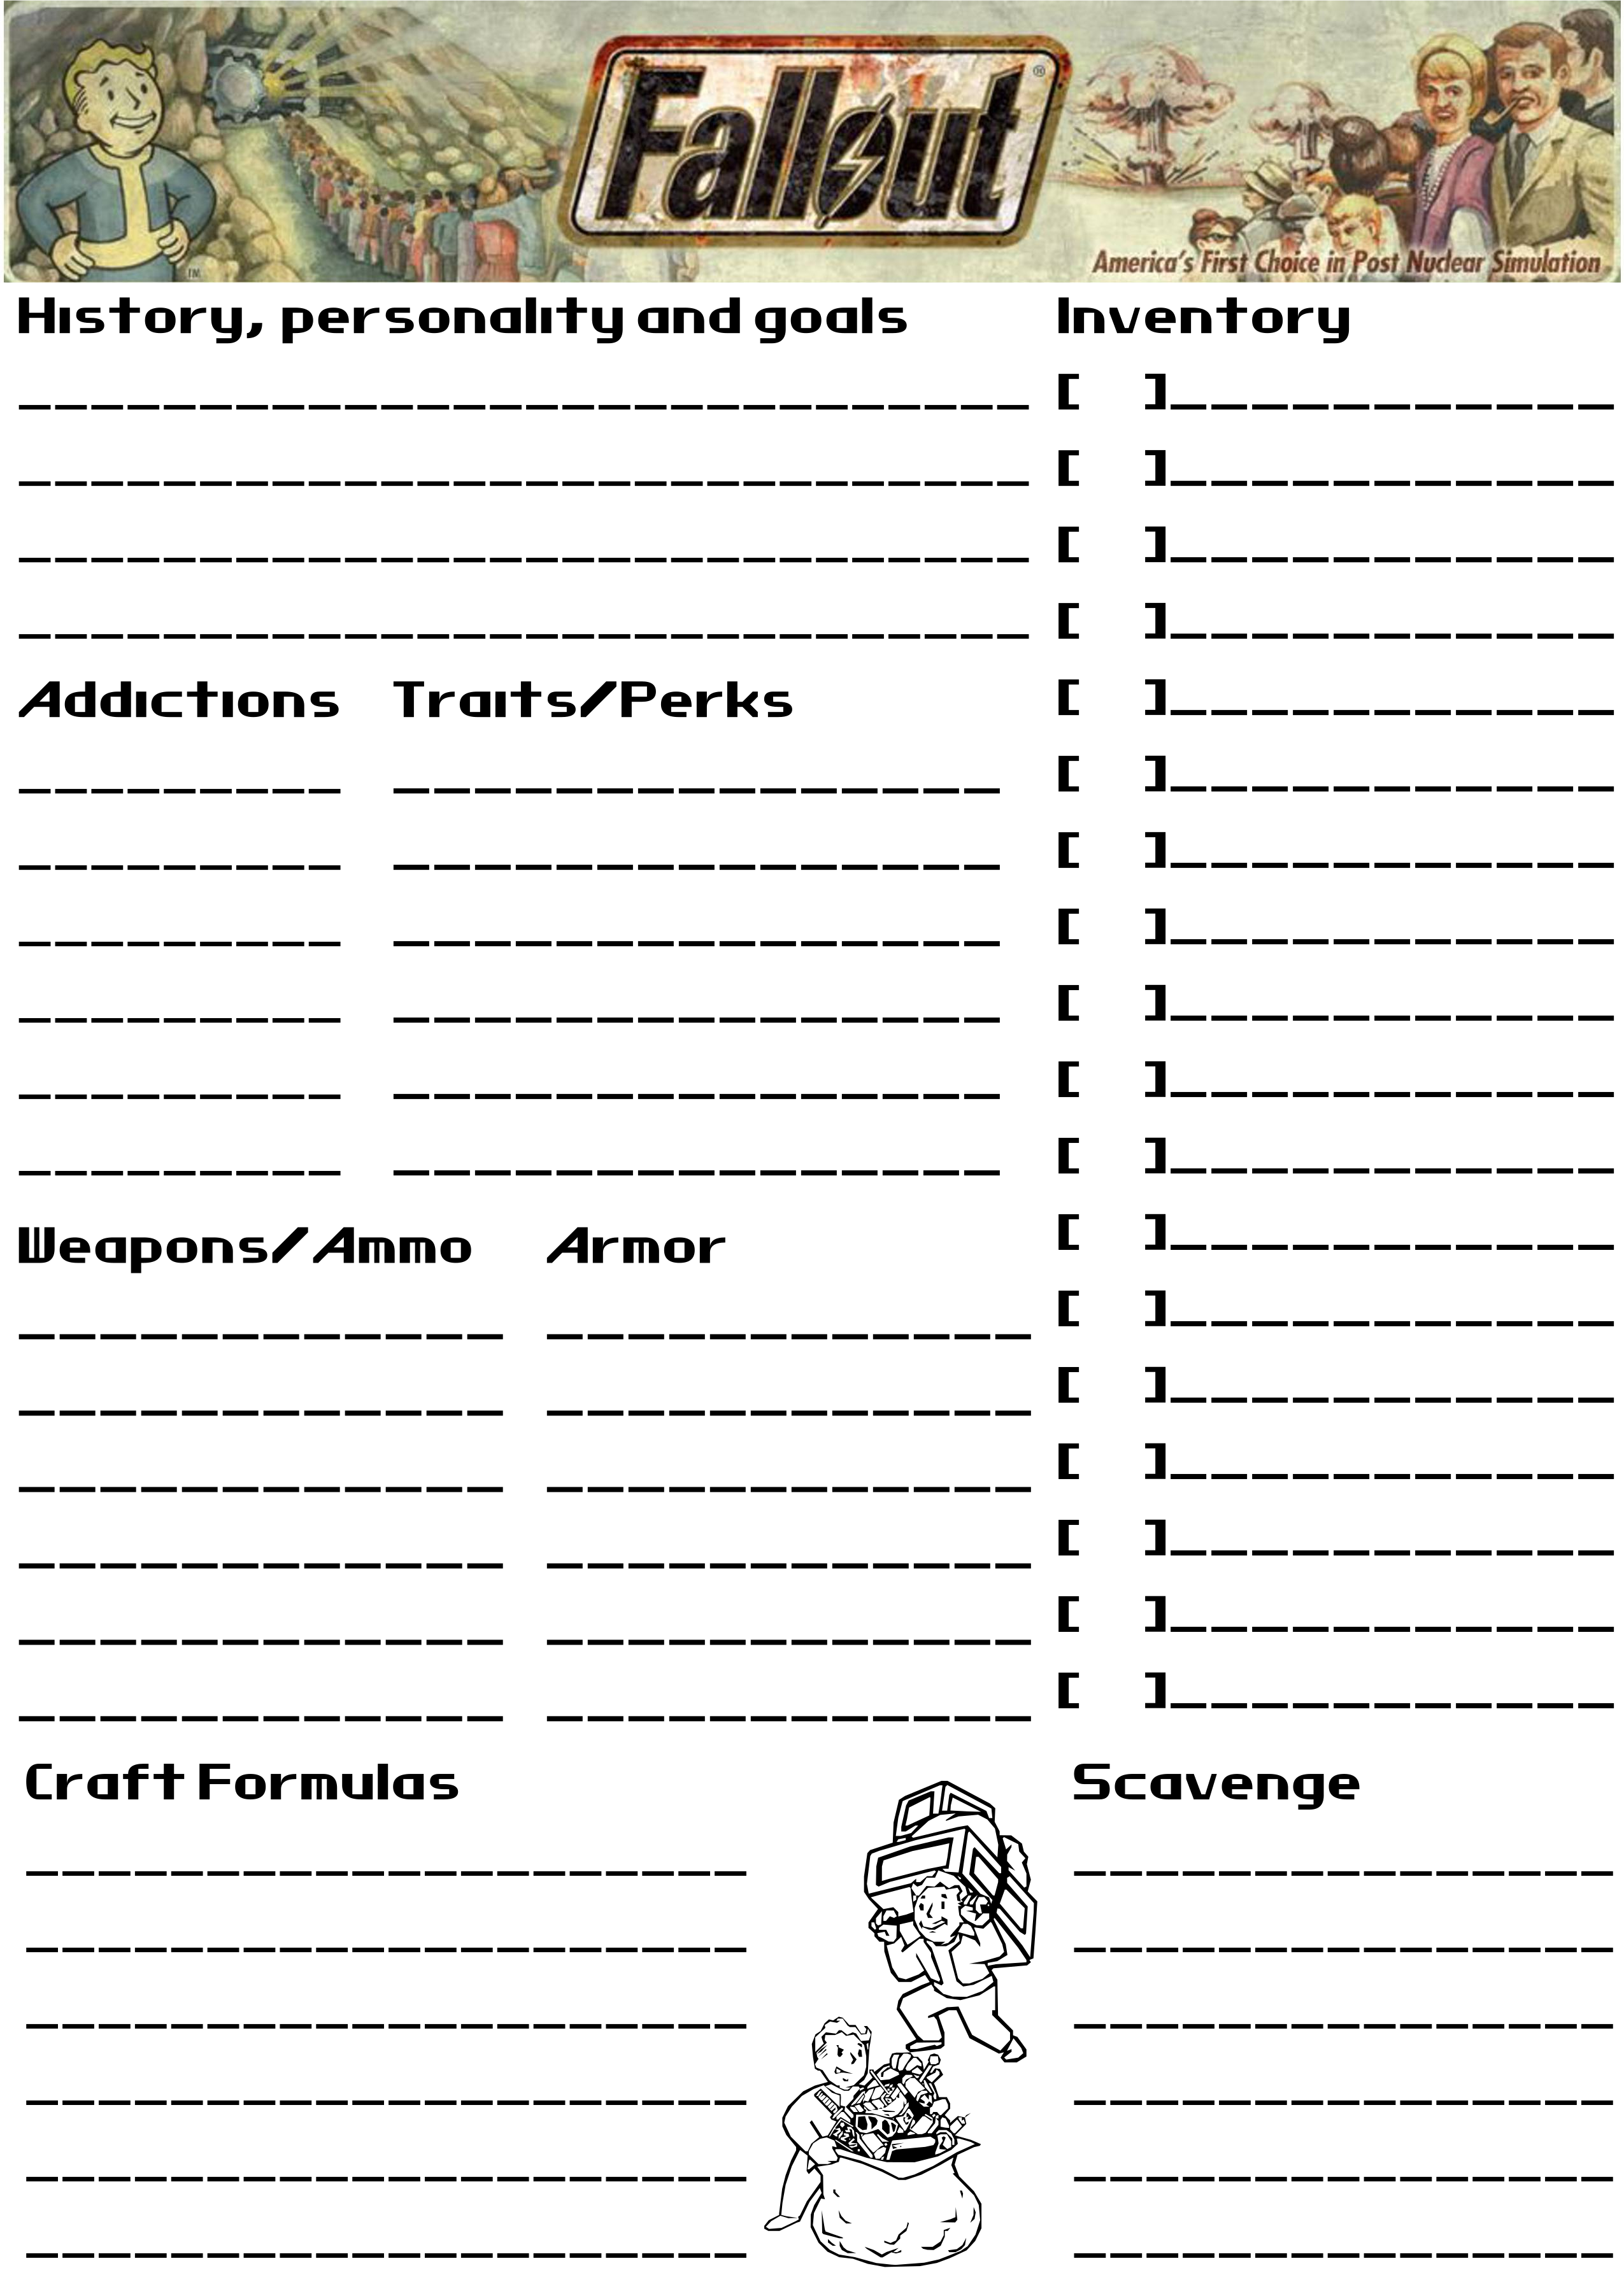
\includegraphics{char_sheet_p2.png}}}
\BgThispage

\begin{Form}

%%%%%%%%%%%%%%%%%%%%%%
%%           HISTORY, PERSONALITY AND GOALS
%%%%%%%%%%%%%%%%%%%%%%

\begin{textblock}{3}(0.01, 2.27)
\TextField[maxlen=400,align=2,height=15pt,width=370pt,name=history1]{}
\end{textblock}

\begin{textblock}{3}(0.01, 2.81)
\TextField[maxlen=400,align=2,height=15pt,width=370pt,name=history2]{}
\end{textblock}

\begin{textblock}{3}(0.01, 3.34)
\TextField[maxlen=400,align=2,height=15pt,width=370pt,name=history3]{}
\end{textblock}

\begin{textblock}{3}(0.01, 3.88)
\TextField[maxlen=400,align=2,height=15pt,width=370pt,name=history4]{}
\end{textblock}

%%%%%%%%%%%%%%%%%%%%%%
%%           ADDICTIONS
%%%%%%%%%%%%%%%%%%%%%%

\begin{textblock}{3}(0.01,4.93)
\TextField[maxlen=100,align=2,height=15pt,width=118pt,name=addictions1]{}
\end{textblock}

\begin{textblock}{3}(0.01,5.48)
\TextField[maxlen=100,align=2,height=15pt,width=118pt,name=addictions2]{}
\end{textblock}

\begin{textblock}{3}(0.01,6.03)
\TextField[maxlen=100,align=2,height=15pt,width=118pt,name=addictions3]{}
\end{textblock}

\begin{textblock}{3}(0.01,6.58)
\TextField[maxlen=100,align=2,height=15pt,width=118pt,name=addictions4]{}
\end{textblock}

\begin{textblock}{3}(0.01,7.09)
\TextField[maxlen=100,align=2,height=15pt,width=118pt,name=addictions5]{}
\end{textblock}

\begin{textblock}{3}(0.01,7.66)
\TextField[maxlen=100,align=2,height=15pt,width=118pt,name=addictions6]{}
\end{textblock}

%%%%%%%%%%%%%%%%%%%%%%
%%           TRAITS/PERKS
%%%%%%%%%%%%%%%%%%%%%%

\begin{textblock}{3}(3.7,4.93)
\TextField[maxlen=400,align=2,height=15pt,width=223pt,name=traitsperks1]{}
\end{textblock}

\begin{textblock}{3}(3.7,5.48)
\TextField[maxlen=400,align=2,height=15pt,width=223pt,name=traitsperks2]{}
\end{textblock}

\begin{textblock}{3}(3.7,6.03)
\TextField[maxlen=400,align=2,height=15pt,width=223pt,name=traitsperks3]{}
\end{textblock}

\begin{textblock}{3}(3.7,6.58)
\TextField[maxlen=400,align=2,height=15pt,width=223pt,name=traitsperks4]{}
\end{textblock}

\begin{textblock}{3}(3.7,7.09)
\TextField[maxlen=400,align=2,height=15pt,width=223pt,name=traitsperks5]{}
\end{textblock}

\begin{textblock}{3}(3.7,7.66)
\TextField[maxlen=400,align=2,height=15pt,width=223pt,name=traitsperks6]{}
\end{textblock}

\begin{textblock}{3}(3.7,6.03)
\TextField[maxlen=400,align=2,height=15pt,width=223pt,name=traitsperks7]{}
\end{textblock}

%%%%%%%%%%%%%%%%%%%%%%
%%           WEAPONS/AMMO
%%%%%%%%%%%%%%%%%%%%%%

\begin{textblock}{3}(0.01, 8.8)
\TextField[maxlen=400,align=2,height=15pt,width=180pt,name=weapons1]{}
\end{textblock}

\begin{textblock}{3}(0.01, 9.34)
\TextField[maxlen=400,align=2,height=15pt,width=180pt,name=weapons2]{}
\end{textblock}

\begin{textblock}{3}(0.01, 9.88)
\TextField[maxlen=400,align=2,height=15pt,width=180pt,name=weapons3]{}
\end{textblock}

\begin{textblock}{3}(0.01, 10.41)
\TextField[maxlen=400,align=2,height=15pt,width=180pt,name=weapons4]{}
\end{textblock}

\begin{textblock}{3}(0.01, 10.93)
\TextField[maxlen=400,align=2,height=15pt,width=180pt,name=weapons5]{}
\end{textblock}

\begin{textblock}{3}(0.01, 11.45)
\TextField[maxlen=400,align=2,height=15pt,width=180pt,name=weapons6]{}
\end{textblock}

%%%%%%%%%%%%%%%%%%%%%%
%%           ARMOR
%%%%%%%%%%%%%%%%%%%%%%

\begin{textblock}{3}(5.2, 8.8)
\TextField[maxlen=400,align=2,height=15pt,width=180pt,name=armor1]{}
\end{textblock}

\begin{textblock}{3}(5.2, 9.34)
\TextField[maxlen=400,align=2,height=15pt,width=180pt,name=armor2]{}
\end{textblock}

\begin{textblock}{3}(5.2, 9.88)
\TextField[maxlen=400,align=2,height=15pt,width=180pt,name=armor3]{}
\end{textblock}

\begin{textblock}{3}(5.2, 10.41)
\TextField[maxlen=400,align=2,height=15pt,width=180pt,name=armor4]{}
\end{textblock}

\begin{textblock}{3}(5.2, 10.93)
\TextField[maxlen=400,align=2,height=15pt,width=180pt,name=armor5]{}
\end{textblock}

\begin{textblock}{3}(5.2, 11.45)
\TextField[maxlen=400,align=2,height=15pt,width=180pt,name=armor6]{}
\end{textblock}


%%%%%%%%%%%%%%%%%%%%%%
%%           SCAVENGE
%%%%%%%%%%%%%%%%%%%%%%

\begin{textblock}{3}(10.45, 12.54)
\TextField[maxlen=400,align=2,height=15pt,width=200pt,name=scavenge1]{}
\end{textblock}

\begin{textblock}{3}(10.45, 13.1)
\TextField[maxlen=400,align=2,height=15pt,width=200pt,name=scavenge2]{}
\end{textblock}

\begin{textblock}{3}(10.45, 13.59)
\TextField[maxlen=400,align=2,height=15pt,width=200pt,name=scavenge3]{}
\end{textblock}

\begin{textblock}{3}(10.45, 14.16)
\TextField[maxlen=400,align=2,height=15pt,width=200pt,name=scavenge4]{}
\end{textblock}

\begin{textblock}{3}(10.45, 14.71)
\TextField[maxlen=400,align=2,height=15pt,width=200pt,name=scavenge5]{}
\end{textblock}

\begin{textblock}{3}(10.45, 15.22)
\TextField[maxlen=400,align=2,height=15pt,width=200pt,name=scavenge6]{}
\end{textblock}


%%%%%%%%%%%%%%%%%%%%%%
%%          CRAFT FORMULAS
%%%%%%%%%%%%%%%%%%%%%%

\begin{textblock}{3}(0.01, 12.54)
\TextField[maxlen=400,align=2,height=15pt,width=270pt,name=craft1]{}
\end{textblock}

\begin{textblock}{3}(0.01, 13.1)
\TextField[maxlen=400,align=2,height=15pt,width=270pt,name=craft2]{}
\end{textblock}

\begin{textblock}{3}(0.01, 13.59)
\TextField[maxlen=400,align=2,height=15pt,width=270pt,name=craft3]{}
\end{textblock}

\begin{textblock}{3}(0.01, 14.16)
\TextField[maxlen=400,align=2,height=15pt,width=270pt,name=craft4]{}
\end{textblock}

\begin{textblock}{3}(0.01, 14.71)
\TextField[maxlen=400,align=2,height=15pt,width=270pt,name=craft5]{}
\end{textblock}

\begin{textblock}{3}(0.01, 15.22)
\TextField[maxlen=400,align=2,height=15pt,width=270pt,name=craft6]{}
\end{textblock}

%%%%%%%%%%%%%%%%%%%%%%
%%           INVENTORY
%%%%%%%%%%%%%%%%%%%%%%

\begin{textblock}{3}(10.55, 2.28)
\TextField[maxlen=6,align=2,height=15pt,width=21pt,name=invAmt1]{}
\end{textblock}
\begin{textblock}{3}(11.4, 2.28)
\TextField[maxlen=400,align=2,height=15pt,width=163pt,name=invItem1]{}
\end{textblock}

\begin{textblock}{3}(10.55, 2.8)
\TextField[maxlen=6,align=2,height=15pt,width=21pt,name=invAmt2]{}
\end{textblock}
\begin{textblock}{3}(11.4, 2.8)
\TextField[maxlen=400,align=2,height=15pt,width=163pt,name=invItem2]{}
\end{textblock}

\begin{textblock}{3}(10.55, 3.35)
\TextField[maxlen=6,align=2,height=15pt,width=21pt,name=invAmt3]{}
\end{textblock}
\begin{textblock}{3}(11.4, 3.35)
\TextField[maxlen=400,align=2,height=15pt,width=163pt,name=invItem3]{}
\end{textblock}

\begin{textblock}{3}(10.55, 3.89)
\TextField[maxlen=6,align=2,height=15pt,width=21pt,name=invAmt4]{}
\end{textblock}
\begin{textblock}{3}(11.4, 3.89)
\TextField[maxlen=400,align=2,height=15pt,width=163pt,name=invItem4]{}
\end{textblock}

\begin{textblock}{3}(10.55, 4.37)
\TextField[maxlen=6,align=2,height=15pt,width=21pt,name=invAmt5]{}
\end{textblock}
\begin{textblock}{3}(11.4, 4.37)
\TextField[maxlen=400,align=2,height=15pt,width=163pt,name=invItem5]{}
\end{textblock}

\begin{textblock}{3}(10.55, 4.93)
\TextField[maxlen=6,align=2,height=15pt,width=21pt,name=invAmt6]{}
\end{textblock}
\begin{textblock}{3}(11.4, 4.93)
\TextField[maxlen=400,align=2,height=15pt,width=163pt,name=invItem6]{}
\end{textblock}

\begin{textblock}{3}(10.55, 5.46)
\TextField[maxlen=6,align=2,height=15pt,width=21pt,name=invAmt7]{}
\end{textblock}
\begin{textblock}{3}(11.4, 5.46)
\TextField[maxlen=400,align=2,height=15pt,width=163pt,name=invItem7]{}
\end{textblock}

\begin{textblock}{3}(10.55, 5.99)
\TextField[maxlen=6,align=2,height=15pt,width=21pt,name=invAmt8]{}
\end{textblock}
\begin{textblock}{3}(11.4, 5.99)
\TextField[maxlen=400,align=2,height=15pt,width=163pt,name=invItem8]{}
\end{textblock}

\begin{textblock}{3}(10.55, 6.54)
\TextField[maxlen=6,align=2,height=15pt,width=21pt,name=invAmt9]{}
\end{textblock}
\begin{textblock}{3}(11.4, 6.54)
\TextField[maxlen=400,align=2,height=15pt,width=163pt,name=invItem9]{}
\end{textblock}

\begin{textblock}{3}(10.55, 7.09)
\TextField[maxlen=6,align=2,height=15pt,width=21pt,name=invAmt10]{}
\end{textblock}
\begin{textblock}{3}(11.4, 7.09)
\TextField[maxlen=400,align=2,height=15pt,width=163pt,name=invItem10]{}
\end{textblock}

\begin{textblock}{3}(10.55, 7.6)
\TextField[maxlen=6,align=2,height=15pt,width=21pt,name=invAmt11]{}
\end{textblock}
\begin{textblock}{3}(11.4, 7.6)
\TextField[maxlen=400,align=2,height=15pt,width=163pt,name=invItem11]{}
\end{textblock}

\begin{textblock}{3}(10.55, 8.14)
\TextField[maxlen=6,align=2,height=15pt,width=21pt,name=invAmt12]{}
\end{textblock}
\begin{textblock}{3}(11.4, 8.14)
\TextField[maxlen=400,align=2,height=15pt,width=163pt,name=invItem12]{}
\end{textblock}

\begin{textblock}{3}(10.55, 8.68)
\TextField[maxlen=6,align=2,height=15pt,width=21pt,name=invAmt13]{}
\end{textblock}
\begin{textblock}{3}(11.4, 8.68)
\TextField[maxlen=400,align=2,height=15pt,width=163pt,name=invItem13]{}
\end{textblock}

\begin{textblock}{3}(10.55, 9.23)
\TextField[maxlen=6,align=2,height=15pt,width=21pt,name=invAmt14]{}
\end{textblock}
\begin{textblock}{3}(11.4, 9.23)
\TextField[maxlen=400,align=2,height=15pt,width=163pt,name=invItem14]{}
\end{textblock}

\begin{textblock}{3}(10.55, 9.78)
\TextField[maxlen=6,align=2,height=15pt,width=21pt,name=invAmt15]{}
\end{textblock}
\begin{textblock}{3}(11.4, 9.78)
\TextField[maxlen=400,align=2,height=15pt,width=163pt,name=invItem15]{}
\end{textblock}

\begin{textblock}{3}(10.55, 10.3)
\TextField[maxlen=6,align=2,height=15pt,width=21pt,name=invAmt16]{}
\end{textblock}
\begin{textblock}{3}(11.4, 10.3)
\TextField[maxlen=400,align=2,height=15pt,width=163pt,name=invItem16]{}
\end{textblock}

\begin{textblock}{3}(10.55, 10.84)
\TextField[maxlen=6,align=2,height=15pt,width=21pt,name=invAmt17]{}
\end{textblock}
\begin{textblock}{3}(11.4, 10.84)
\TextField[maxlen=400,align=2,height=15pt,width=163pt,name=invItem17]{}
\end{textblock}

\begin{textblock}{3}(10.55, 11.38)
\TextField[maxlen=6,align=2,height=15pt,width=21pt,name=invAmt18]{}
\end{textblock}
\begin{textblock}{3}(11.4, 11.38)
\TextField[maxlen=400,align=2,height=15pt,width=163pt,name=invItem18]{}
\end{textblock}


\end{Form}

\end{document}
